\documentclass[10pt,a4paper]{report} 

\usepackage[utf8]{inputenc}
\usepackage{amsmath}
\usepackage{amsfonts}
\usepackage{amssymb}
\usepackage{graphicx}
\usepackage[final]{pdfpages}
\usepackage{stmaryrd}
\usepackage{listings}
\usepackage[hidelinks]{hyperref}
\usepackage[english]{babel}
\usepackage{color}
\usepackage{fancyhdr}
\usepackage{xcolor}
\usepackage{url}
\usepackage{sectsty}
\usepackage{etoolbox}
\usepackage{tikz}
\usepackage[acronym]{glossaries}
\usepackage{float}
\usepackage[bottom]{footmisc}
\usepackage[parfill]{parskip}
\usepackage{mathrsfs}
\usepackage{algpseudocode}
\usepackage{algorithm}
\usepackage{bbm}

% Abstract
\patchcmd{\abstract}{\null\vfil}{}{}{}

% Graphics and images
\graphicspath{{./images/}}

% Set headers to sans serif
\allsectionsfont{\sffamily}

% Defining colors for syntax highlighting
\definecolor{commentsColor}{rgb}{0.497495, 0.497587, 0.497464}
\definecolor{keywordsColor}{rgb}{0.000000, 0.000000, 0.635294}
\definecolor{stringColor}{rgb}{0.558215, 0.000000, 0.135316}

\lstset{aboveskip=20pt,belowskip=20pt}

% Source: https://denbeke.be/blog/programming/syntax-highlighting-in-latex/
\lstset{
  backgroundcolor=\color{white},
  basicstyle=\ttfamily\small,
  breakatwhitespace=false,
  breaklines=true,
  captionpos=b,
  commentstyle=\color{commentsColor}\textit,
  deletekeywords={...},
  escapeinside={\%*}{*)},
  extendedchars=true,
  frame=tb,
  keepspaces=true,
  keywordstyle=\color{keywordsColor}\bfseries,
  %language=Python,
  otherkeywords={*,...},
  %numbers=left,
  numbersep=5pt,
  numberstyle=\tiny\color{commentsColor}, 
  rulecolor=\color{black}, 
  showspaces=false,
  showstringspaces=false,
  showtabs=false, 
  stepnumber=1, 
  stringstyle=\color{stringColor},
  tabsize=2, 
  title=\lstname,
  columns=fixed 
}

% Bibliography
\bibliographystyle{unsrturl}

% Pagestyle
\pagestyle{fancy}

% Hyperlinks
\hypersetup{
  colorlinks=true,
  allcolors=black
}

% Headers
\fancyhf{}
\lhead[\textit{\leftmark}]{}
\rhead[]{\textit{\leftmark}}

\begin{document}

\title{
\vspace{-80px}

\includegraphics[width=5cm]{bfh-logo}\\
\vspace{80px}
\huge\textsf{\textbf{3D Terrain with Level of Detail}}\\
\vspace{50px}
\large{Written report for the module\\
BTI3041 -- Project 2\\ 
by\\}
\vspace{20px}
\Large{Amar Tabakovic\\}
\vspace{40px}
\large{
\textbf{Bern University of Applied Sciences}\\
  Engineering and Information Technology\\
  Computer Perception \& Virtual Reality Lab
\\
\vspace{20px}
\textbf{Supervisor}\\
Prof. Marcus Hudritsch}\\
\vspace{30px}
\today
}
%\author{
%  Amar Tabakovic
%}
\date{}
\maketitle

\begin{abstract}
Rendering terrains is a central task for video games, geographic information systems and simulators, 
but also computationally expensive. Optimizations, one of which is the level of detail (LOD),
are necessary in order to ensure appropriate performances.
This project aims to give an overview of the topic of terrain rendering.
As part of this project, a demo terrain renderer (ATLOD) was implemented in C++ and OpenGL.
ATLOD currently supports naive brute-force rendering, GeoMipMapping, TODO.

\end{abstract}
%\chapter*{Acknowledgements}
%\thispagestyle{empty}
%I would like to thank my dear
%\clearpage

\tableofcontents

\chapter{Introduction}
In 3D computer graphics, rendering is the central task.
Many practical applications of 3D computer graphics make use of terrains, 
such as flight simulators, open-world video games, and Geographic Information Systems (GIS) \cite[p.~185]{lodfor3dgraphics}.
At the same time, rendering terrains, which are large and constantly visible, is computationally expensive 
and optimizations are necessary in order to ensure adequate performance.

One area which offers potential for optimizations is the \textit{level of detail (LOD)}.
The concept of LOD is based on the intuitive idea that the farther away an object is, the fewer details are going to be visible to the human eye.
Over the last three decades, numerous algorithms and approaches have been published 
for the problem of efficient terrain rendering.

\section{Goals of this Project}
The primary goal of this project is the study and exploration
of terrain rendering algorithms.
First, the basics of terrain rendering are studied and 
an overview of the state-of-the-art of terrain rendering is 
constructed. Afterwards, a demo terrain renderer is developed,
using the ideas from one or more of the evaluated algorithms.

This project is restricted to simple heightmap rendering, without any real-time 
streaming/paging of terrain data.

\section{Intended Readership}
The reader is assumed to be familiar with the basics of computer graphics, C++ and OpenGL.

\section{Notation and Terminology}
\subsection{Mathematical Notation}
This report uses the following mathematical notation:
\begin{itemize}
      \item The coordinate system is a right-handed coordinate system with $y$ as the up-direction, unless explicitly stated otherwise.
      \item $\mathbb{N}$ denotes the set of natural numbers, $\mathbb{R}$ is the set of real numbers, $\mathbb{R}^n$ is the set of real numbers in $n$ dimensions.
      \item $\mathbf{p} = (p_x, p_y, p_z)$ denotes a point in $\mathbb{R}^3$.
      \item $\mathbf{v} = (v_x, v_y, v_z)$ denotes a vector in $\mathbb{R}^3$.
      \item $\mathbf{M}$ denotes a matrix in $\mathbb{R}^{n \times n}$.
\end{itemize}

\subsection{The Term ``LOD Level''}
The definition of what ``LOD level 0'' and what ``LOD level $l$'' ($l = $ maximum LOD) mean is different from paper to paper.
Normally, LOD systems use 0 for the highest resolution and $l$ for the lowest resolution.
In this report, the opposite (and slightly more intuitive) approach is followed: $l$ denotes the highest resolution, and 0 denotes the lowest resolution.

\section{Outline of the Report}
This report is structured as follows:
\begin{itemize}
  \item Chapter 2 introduces the reader to the basics of terrain rendering. The topics covered include 
        terrain data representation, common optimizations and potential problems during rendering.
  \item Chapter 3 gives an overview of the state of the art of terrain rendering.
        Various algorithms and their central ideas are presented in a high-level manner.
        Afterwards, some examples of real-world systems using terrain LOD algorithms are listed.
  \item Chapter 4 describes the demo terrain renderer (named ATLOD) which was developed.
        The basic features and the details of the implemented algorithm are presented.
  \item In chapter 5, the performance and visual accuracy of ATLOD is measured and the results documented.
  \item Chapter 6 gives a short discussion of the results from chapter 5.
  \item Chapter 7 concludes this report by mentioning some potential improvements and the 
        outlook for the bachelor thesis.
\end{itemize}



\chapter{Existing Work and Literature}
\section{Research Articles and Publications}
Terrain LOD is a well-researched topic and over the last three decades, numerous approaches have been published.
TODO: list research

\section{Level of Detail for Computer Graphics}
\textit{Level of Detail for Computer Graphics} by Luebke \textit{et al.} \cite{lodfor3dgraphics} 
is a reference book for the topic of 
LOD published in 2002. The book builds on top of years of research in the 
area of LOD and provides an overview to many LOD techniques. For this project,
chapter 7 ``Terrain Level of Detail'' of the book is especially relevant, 
as it dives into the topic of LOD for terrains specifically.
It covers basic approaches and techniques for terrain LOD, 
common problems that can arise during rendering of terrains and some solutions to them, 
and a catalog of terrain LOD algorithms.

\section{Focus on 3D Terrain Programing}
\textit{Focus on 3D Terrain Programming} by Trent Polack \cite{focuson3dterrainprogramming} is a book on terrain programming published in 2002.
Part one of the book introduces the reader to the basics of terrains, such as height maps and texturing. Part two then 
covers some more advanced topics, including a selection of terrain LOD algorithms. The presented LOD algorithms are
\begin{itemize}
  \item ROAM by Duchaineau \textit{et al.} \cite{roam},
  \item the quadtree-based algorithm described in ``Real-Time Generation of Continuous Levels of Detail for Height Fields'' by Röttger \textit{et al.} \cite{rottgerpaper},
  \item and geomipmapping by de Boer \cite{geomipmapping}.
\end{itemize}
The book also includes demo source code in C++ and OpenGL.

\section{Virtual Terrain Project}
The \textit{Virtual Terrain Project} \cite{vtp} was a project run from 2001 to 2013 
that consisted of a collection of software, information and resources on terrain modelling and rendering,
including a large overview of publications and implementations related to terrain LOD algorithms.

\chapter{Basics of Terrain Rendering}
\section{Terrain Data Representation}
\subsection{Heightmaps}
One way of representing terrains is using \textit{heightmaps}.
A heightmap is a $n\times n$-grid that contains 
the height value $y$ for each $(x,z)$-position.
Positions are always spaced evenly in a grid-like manner,
but the distance between any two neighboring positions (in other words the $(x,z)$-scale) is variable.

The main advantage of heightmaps is that they allow for very simple storage and manipulation of height data, e.g. in form of images,
where low color values represent low areas of terrain and vice versa for
high color values. The color representation of an image influences the number of possible height values:
\begin{itemize}
  \item For an 8-bit grayscale image, 256 height values are supported.
  \item For a 16-bit grayscale image, 65536 height values are supported.
  \item For an 8-bit RGB image, more than 16 million height values are supported. 
\end{itemize}
Retrieving the height value for a given $(x,z)$-position is easy,
which consists of a simple lookup at the given position in the image.
Figure~\ref{fig:dom} shows a $2000 \times 2000$ heightmap of the mountain Dom in Valais, Switzerland.
\begin{figure}[H]
  \centering
  
\includegraphics[width=0.4\textwidth]{dom}
  \caption{$2000 \times 2000$ heightmap of the mountain Dom in Valais, Switzerland retrieved from SwissTopo \cite{alti3d}.}\label{fig:dom}
\end{figure}

\subsection{Triangulated Irregular Networks}
A less commonly used alternative to the heightmap is the \textit{triangulated irregular network (TIN)} data structure.
A TIN consists of a collection of 3-dimensional vertices, where 
the arrangement of vertices can be irregular. Figure~\ref{fig:tin-example} shows 
an example of a TIN.
\begin{figure}[H]
  \centering
  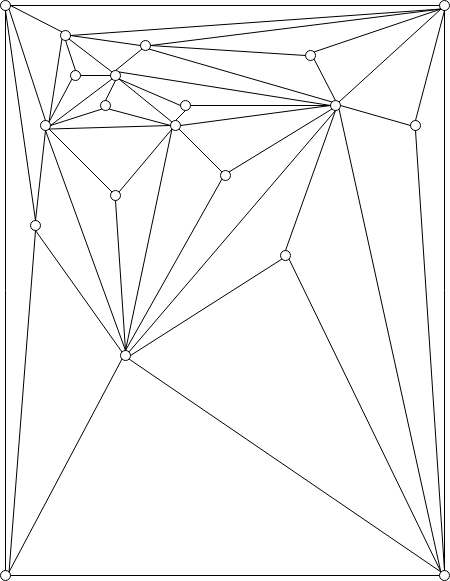
\includegraphics[width=0.52\textwidth]{tin-example}
  \caption{Example of a TIN. Note that the left area represents a terrain area with many changes 
  (e.g. mountains, hills, etc.), and the right area represents an area with few changes (e.g. flat areas).}\label{fig:tin-example}
\end{figure}

The main advantage of TINs is that fewer polygons need to be used for 
e.g. smooth terrain areas. Another advantage is that
special terrain features can be modelled 
which are usually difficult to model with heightmaps, such as overhangs, cliffs and caves \cite{lodfor3dgraphics}.
The disadvantage of TINs, however, is that the full $(x,y,z)$ coordinates need to be stored,
whereas with heightmaps, only the height value $y$ needs to be stored.
Another disadvantage of TINs is that many terrain LOD algorithms work with 
heightmaps, such as \cite{roam,geomipmapping,rottgerpaper,geomclipmaps,gpugeomclipmaps,chunkedlod,cdlod,cbt}, and not with TINs.

\section{Bintrees and Quadtrees}
\textit{Binary triangle trees (bintrees)} and \textit{quadtrees} are 
recursive data structures based on triangles and quads respectively.
Bintrees and quadtrees are mostly found in historical algorithms,
such as \cite{lindstrom1996} and \cite{roam}, but have recently been revitalized in \cite{cbt}.

A bintree consists of up to two child triangles, both of which also consist of up to two child triangles each, and so forth.
Quadtrees are structured similarly, with a quad consisting of up to four child quads, and each child quad consisting
of up to four child quads, and so forth.
Figure~\ref{fig:bintree-quadtree-example} shows an example of a bintree and a quadtree.

\begin{figure}[H]
  \centering
  \subfloat[\centering]{{
\includegraphics[width=0.43\textwidth]{bintree-example} }}
  \qquad
  \subfloat[\centering]{{
\includegraphics[width=0.33\textwidth]{quadtree-example.png} }}%
  \caption{Example of a bintree (a) and a quadtree (b).}\label{fig:bintree-quadtree-example}
\end{figure}

The main advantage of bintrees and quadtrees is that 
LOD can be modelled very naturally with them.
Bintree/quadtree sections with few children correspond to a low LOD and 
vice versa for bintree/quadtree sections with many children.

\section{View-frustum Culling}
\textit{View-frustum culling} is an optimization technique commonly used in computer graphics.
View-frustum culling is used in numerous terrain LOD approaches, such as \cite{lindstrom1996,roam,geomipmapping,geomclipmaps,cdlod}.
The \textit{view-frustum} is the 3-dimensional pyramid that represents the space that is visible to the camera.
It is defined by six planes: the near, far, left, right, top and bottom face.
Each face has a normal vector and a distance from the origin. Figure \ref{fig:view-frustum} 
shows an example of a view frustum.

\begin{figure}[H]
  \centering
  
\includegraphics[width=0.62\textwidth]{view-frustum}
  \caption{Example of a view-frustum}\label{fig:view-frustum}
\end{figure}

The main idea of view-frustum culling is to check whether the \textit{bounding volume} of an object 
is contained (at least partially) inside the view-frustum, and if not, to simply not render the object.
This dramatically reduces the number of draw calls and the number of vertices that get rendered.
The bounding volume of an object is the 3-dimensional volume such that it contains the entire object inside of it.
There are different types of bounding volumes, such as \textit{axis-aligned bounding boxes (AABB)}, \textit{oriented bounding boxes (OBB)},
\textit{bounding spheres}, and more. AABB's are commonly used in terrain LOD algorithms \cite{geomipmapping,geomclipmaps,cdlod}
and are defined with two points $\mathbf{p}_{min}$ and $\mathbf{p}_{max}$, which indicate both endpoints of the AABB.
Figure \ref{fig:aabb-block} shows a terrain block with its AABB in red.

\begin{figure}[H]
  \centering
  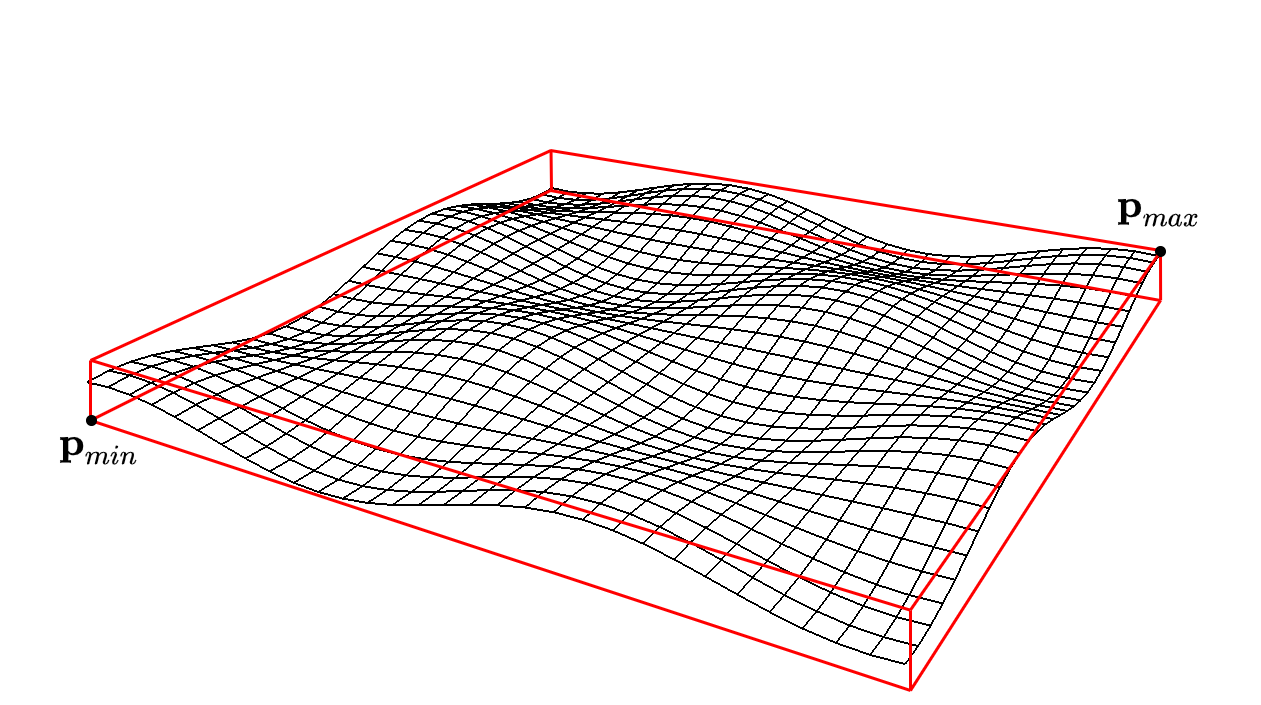
\includegraphics[width=0.72\textwidth]{aabb-block}
  \caption{Example of a terrain block with its AABB defined by $\mathbf{p}_{min}$ and $\mathbf{p}_{max}$, marked in red.}\label{fig:aabb-block}
\end{figure}

View-frustum culling can be further optimized by arranging the scene hierarchy (i.e. the terrain hierarchy)
into a \textit{space-parititioning data structure}. A widely-used structure is the already previously mentioned quadtree, where leaf nodes contain the renderable terrain sections and where
each node has an AABB that contains all bounding volumes of its child nodes.
Note that the quadtree in this case is not the same kind of quadtree from the previous section.
At render time, the quadtree gets traversed starting from the root node.
The intersection of the view-frustum with the AABB of each of the four child nodes gets calculated
and if the AABB of a child node intersects with the view-frustum, the child node gets recursively traversed
and the same steps are performed until reaching a leaf node, at which point the terrain section gets rendered.
The number of AABB-view-frustum-intersection calculations gets reduced, however at the cost of more memory consumption.
Figure \ref{fig:quadtree-frustum-culling} shows an example of quadtree-based view-frustum culling.

\begin{figure}[H]
  \centering
  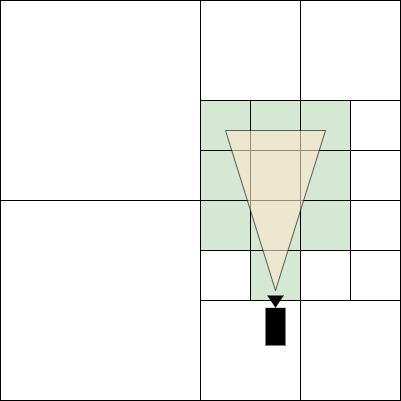
\includegraphics[width=0.4\textwidth]{quadtree-frustum-culling.png}
  \caption{Example of view-frustum culling with a quadtree viewed from the top. The view-frustum is marked in yellow and blocks that intersect the view-frustum are marked in green.}\label{fig:quadtree-frustum-culling}
\end{figure}

\section{Potential Problems During Terrain Rendering}
While terrain LOD algorithms dramatically improve the performance of terrain rendering, 
there are certain issues that can occur. 

\subsection{Cracks}
Cracks and holes in terrains can appear when a higher LOD terrain section is bordered 
by a lower LOD terrain section. The main problem is that when a vertex $v_{\text{high}}$ of a higher LOD terrain section lies on the edge $e_{\text{low}}$
of a lower LOD terrain section and the $y$ coordinate of $v_{\text{high}}$ is greater or less than the 
height of $e_{\text{low}}$ at that point, the difference in height causes the crack to appear, as shown in figure~\ref{fig:crack-example}.
\begin{figure}[H]
  \centering
  \subfloat[\centering The crack is caused by the height difference of $v_{\text{high}}$ and $e_{\text{low}}$.]{{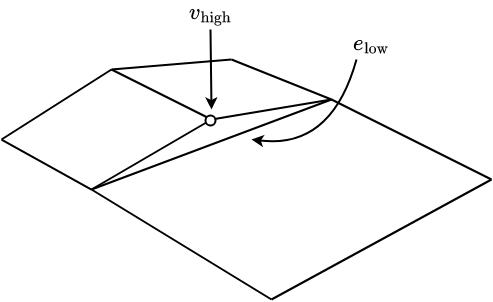
\includegraphics[width=0.5\textwidth]{crack-example} }}
  \qquad
  \subfloat[\centering The background color is set to red to highlight the cracks.]{{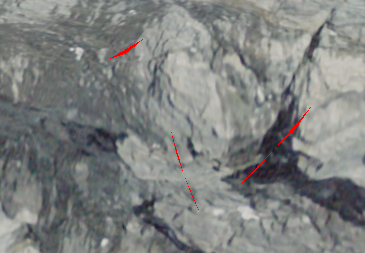
\includegraphics[width=0.4\textwidth]{cracks-terrain} }}%
  \caption{Illustration of a crack (a) and some examples of cracks in a real rendered terrain (b).}\label{fig:crack-example}
\end{figure}
Cracks can be solved by either of the following, depending on the capabilities of the LOD approach:
\begin{itemize}
  \item Removing the vertex in question, causing the higher and lower LOD meshes to be connected seamlessly (in figure~\ref{fig:crack-example} vertex $v_{\text{high}}$).
  \item Inserting an extra vertex at the border edge of the lower LOD mesh \cite[p.~194]{lodfor3dgraphics} (in figure~\ref{fig:crack-example} on top of vertex $v_{\text{high}}$). The disadvantage of this is that an extra vertex needs to get created.
  \item Covering the cracks area by rendering a strip \cite{gpugeomclipmaps}
\end{itemize}

\subsection{Popping}
The phenomenon of \textit{popping} occurs when the camera is moving 
and the transition of the terrain's LOD level causes visual pops to appear.
Popping decreases the realism of the terrain and should be as minimal as possible.
Popping can be reduced with \textit{vertex morphing} \cite{geomipmapping,geomclipmaps,cdlod}, 
i.e. by animating the transition of one LOD level to the next seamlessly through interpolation.
\chapter{Algorithms and Approaches for Terrain LOD}
\section{ROAM}
\textit{ROAM} (short for \textbf{R}eal-time \textbf{O}ptimally \textbf{A}dapting \textbf{M}eshes) 
is a terrain LOD algorithm developed by Duchaineau \textit{et al.} \cite{roam} published in 1997.
ROAM represents the terrain mesh using bintrees and performs triangle splits and merges
for generating and removing detail. 
The splits and merges happen mainly on the CPU, which makes ROAM a mainly CPU-based approach.

\subsection{General Idea}
The central idea of the algorithm is to use temporal coherence: the mesh from a previous frame $\mathbf{T}_{f-1}$ is used to compute 
the mesh of the current frame $\mathbf{T}$, rather than building up the mesh from ground up for each frame.
This is done using two priority queues: a split queue $\mathcal{Q}_s$ and a merge queue $\mathcal{Q}_m$.
The split queue contains splittable triangles $T$
and the merge queue contains mergable triangle pairs $(T,T_B)$.
The elements of the priority queues are ordered by 
various geometric error metrics, which are explained in the subsection ``Error Metrics'' of this report.
At each frame, the terrain mesh gets split and merged using $\mathcal{Q}_s$ and $\mathcal{Q}_m$. until either the required size/accuracy is reached
or the time runs out.
ROAM is designed as a greedy algorithm, meaning it will always performs the most optimal splits/merges for each frame.

\subsection{Error Metrics}
The original ROAM paper mentions various error metrics for the priority queue ordering,
which are explained in the following paragraphs.

\paragraph{Wedgies} \textit{Wedgies} are nested bounding volumes around triangles that are computed 
while building the initial mesh at the beginning of the algorithm.
A wedgie is defined to contain the entire $x$ and $z$ extent\footnote{The original ROAM paper uses $z$ for the up direction. For the sake of consistency with the rest of this report, we will use $y$ as the up direction here.}
of a triangle and the height $y$ including some additional space above and below the highest and lowest points,
respectively.

\paragraph{Geometric Screen Distortion}
Another metric is the distance between where a node is supposed to be on the screen and where the algorithm placed the node.
The maximum of all distances is calculated and used as the base priority metric of the algorithm.

\subsection{Other Optimizations}
\paragraph{View-frustum Culling}
An optimization that is mentioned is view-frustum culling. In each frame, various flags are updated during 
the recursive traversal of the bintree. These flags indicate whether a wedgie is inside the view-frustum 
fully, partially, or not at all.

\paragraph{Incremental Triangle Stripping}
The ROAM paper reports using \textit{incremental triangle stripping} for optimizing the performance of the rendering.
This is simply refers to using triangle strips for rendering. which is supported by all major graphics APIs.

\subsection{Conclusion}
The runtime of ROAM is independent of the screen resolution and is proportional to the 
number of triangle changes per frame. 

%\section{Röttger's Quadtree-based Algorithm}
%TODO

\section{GeoMipMapping}
\textit{Geometrical Mipmapping (GeoMipMapping)} is a terrain LOD approach developed by de Boer \cite{geomipmapping} in the year 2000. 
It applies the idea of texture mipmapping to terrain rendering. In this section, all 
presented ideas are from the original paper, unless noted otherwise.

\subsection{General Idea}
The central idea of GeoMipMapping is its analogy to texture mipmapping: just like how textures of far away objects are rendered using lower resolution texture mipmaps,
terrain areas that are far away from the camera should also be rendered with a lower resolution mesh.

This is achieved by splitting up the terrain into so-called \textit{blocks} (also called \textit{patches}) of a fixed width $2^n + 1$ for an arbitrary $n \in \mathbb{N}$.
Each block has a LOD level\footnote{The original GeoMipMapping paper uses 0 to denote the maximum LOD level and vice-versa for the minimum LOD level. In order to avoid any confusion with the term \textit{LOD}, this report denotes 0 as the minimum LOD level and vice versa for the maximum LOD level.} $0\leq l \leq n$ that changes dynamically at runtime.
At load time, every block is computed at every LOD level and subsequently stored, e.g. on an index buffer.
Each such representation of a block at a specific LOD level is called a \textit{GeoMipMap}.
For each GeoMipMap, the number of vertices on one side is $2^{l}+1$ and the number of quads is $2^{2l}$.

For example, the GeoMipMaps of a $5 \times 5$ terrain block contain $2^2 + 1 = 5$ vertices on one side at the maximum LOD level 2, $2^1 + 1 = 3$ vertices at LOD level 1 and $2^0 + 1 = 2$ vertices at the minimum LOD level 0.
As for the number of quads, at LOD level 2 there are $2^{4} = 16$ quads, at LOD level 1 there are $2^2 = 4$ quads and at LOD level 0 there is $2^0 = 1$ quad.
Figure~\ref{fig:geomipmapping-patch-example} illustrates the above example.

% \begin{figure}[H]
%   \centering
%   
\includegraphics[width=1\textwidth]{geomipmapping-patch-example}
%   \caption{Example of a $5 \times 5$ block at the maximum LOD level of 2 (left), LOD level of 1 (middle) and minimum LOD level of 0 (right). The omitted vertices of the lower LOD blocks are shown here as dotted circles.}\label{fig:geomipmapping-patch-example}
% \end{figure}

\begin{figure}[H]
  \centering
  \subfloat[\centering LOD level 2 (maximum).]{{
\includegraphics[width=0.28\textwidth]{geomipmapping-level-2.png} }}
  \qquad
  \subfloat[\centering LOD level 1.]{{
\includegraphics[width=0.28\textwidth]{geomipmapping-level-1.png} }}
  \qquad
  \subfloat[\centering LOD level 0 (minimum).]{{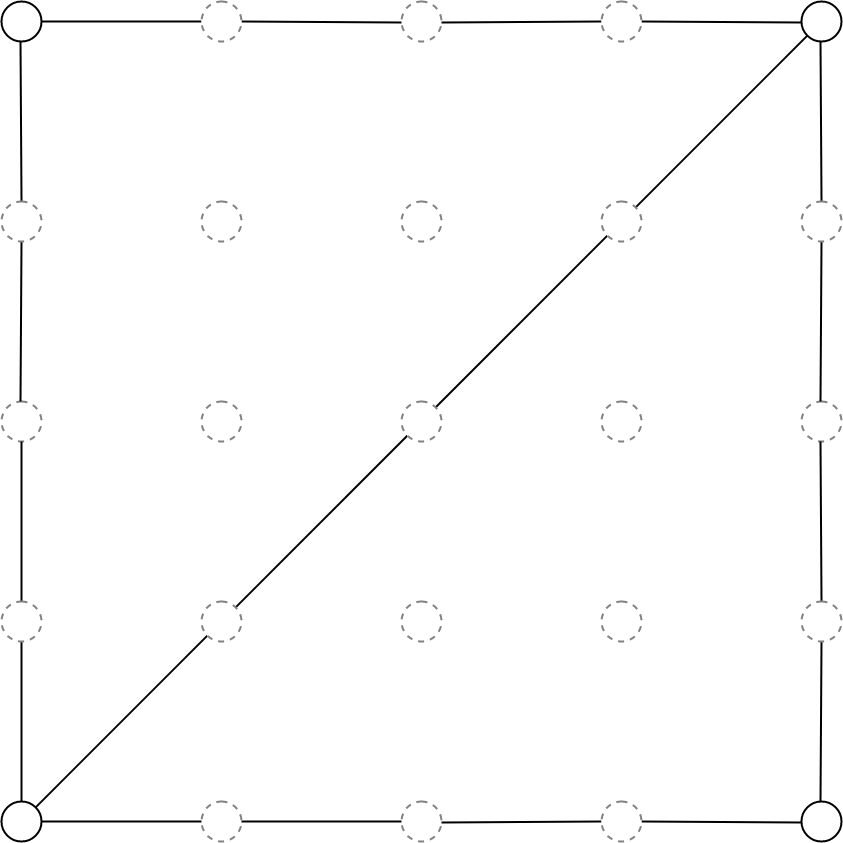
\includegraphics[width=0.28\textwidth]{geomipmapping-level-0.png} }}
  \caption{Example of each GeoMipMap of a $5 \times 5$ block. The omitted vertices of lower LOD GeoMipMaps are marked as dotted circles.}\label{fig:geomipmapping-patch-example}
\end{figure}

\subsection{View-frustum Culling}
The organisation of the terrain into blocks allows for easy view-frustum culling,
which dramatically decreases the number of vertices that need to get rendered.


\subsection{LOD Selection}
The LOD for each block is selected at runtime and is based on a 

\subsection{Avoiding Cracks}
GeoMipMapping avoids cracks by checking whether the
current block has a higher LOD than the bordering block and if this is the case,
it omits the vertices that would cause the crack.
The vertex omission is performed by rendering the bordering row/column of the current block
as triangle fans, as shown in figure~\ref{fig:geomipmapping-crack-avoidance}.

\begin{figure}[H]
  \centering
  
\includegraphics[width=0.7\textwidth]{geomipmapping-crack-avoidance}
  \caption{Example of GeoMipMapping's crack avoidance between a LOD 2 and a LOD 1 GeoMipMap of two $5 \times 5$ blocks as described in the original paper.}\label{fig:geomipmapping-crack-avoidance}
\end{figure}

% An alternative way to render neighboring blocks with different LOD levels is to render the triangle fans from the center point of each $3 \times 3$ border subblock. 
% This approach is somewhat simpler for handling special cases, e.g. when both the top and right neighboring blocks have a lower LOD,
% as shown shown in figure~\ref{fig:geomipmapping-crack-avoidance-alternative}.

%\begin{figure}[H]
%  \centering
%  \includegraphics[width=0.5\textwidth]{geomipmapping-crack-avoidance-alternative}
%  \caption{Alternative method to avoid cracks between a LOD 2 and a LOD 1 GeoMipMap of two $5 \times 5$ blocks.}\label{fig:geomipmapping-crack-avoidance-alternative}
%\end{figure}

\begin{figure}[H]
  \centering
  \subfloat[\centering Using the entire $3\times 3$ border subblocks for the triangle fans.]{{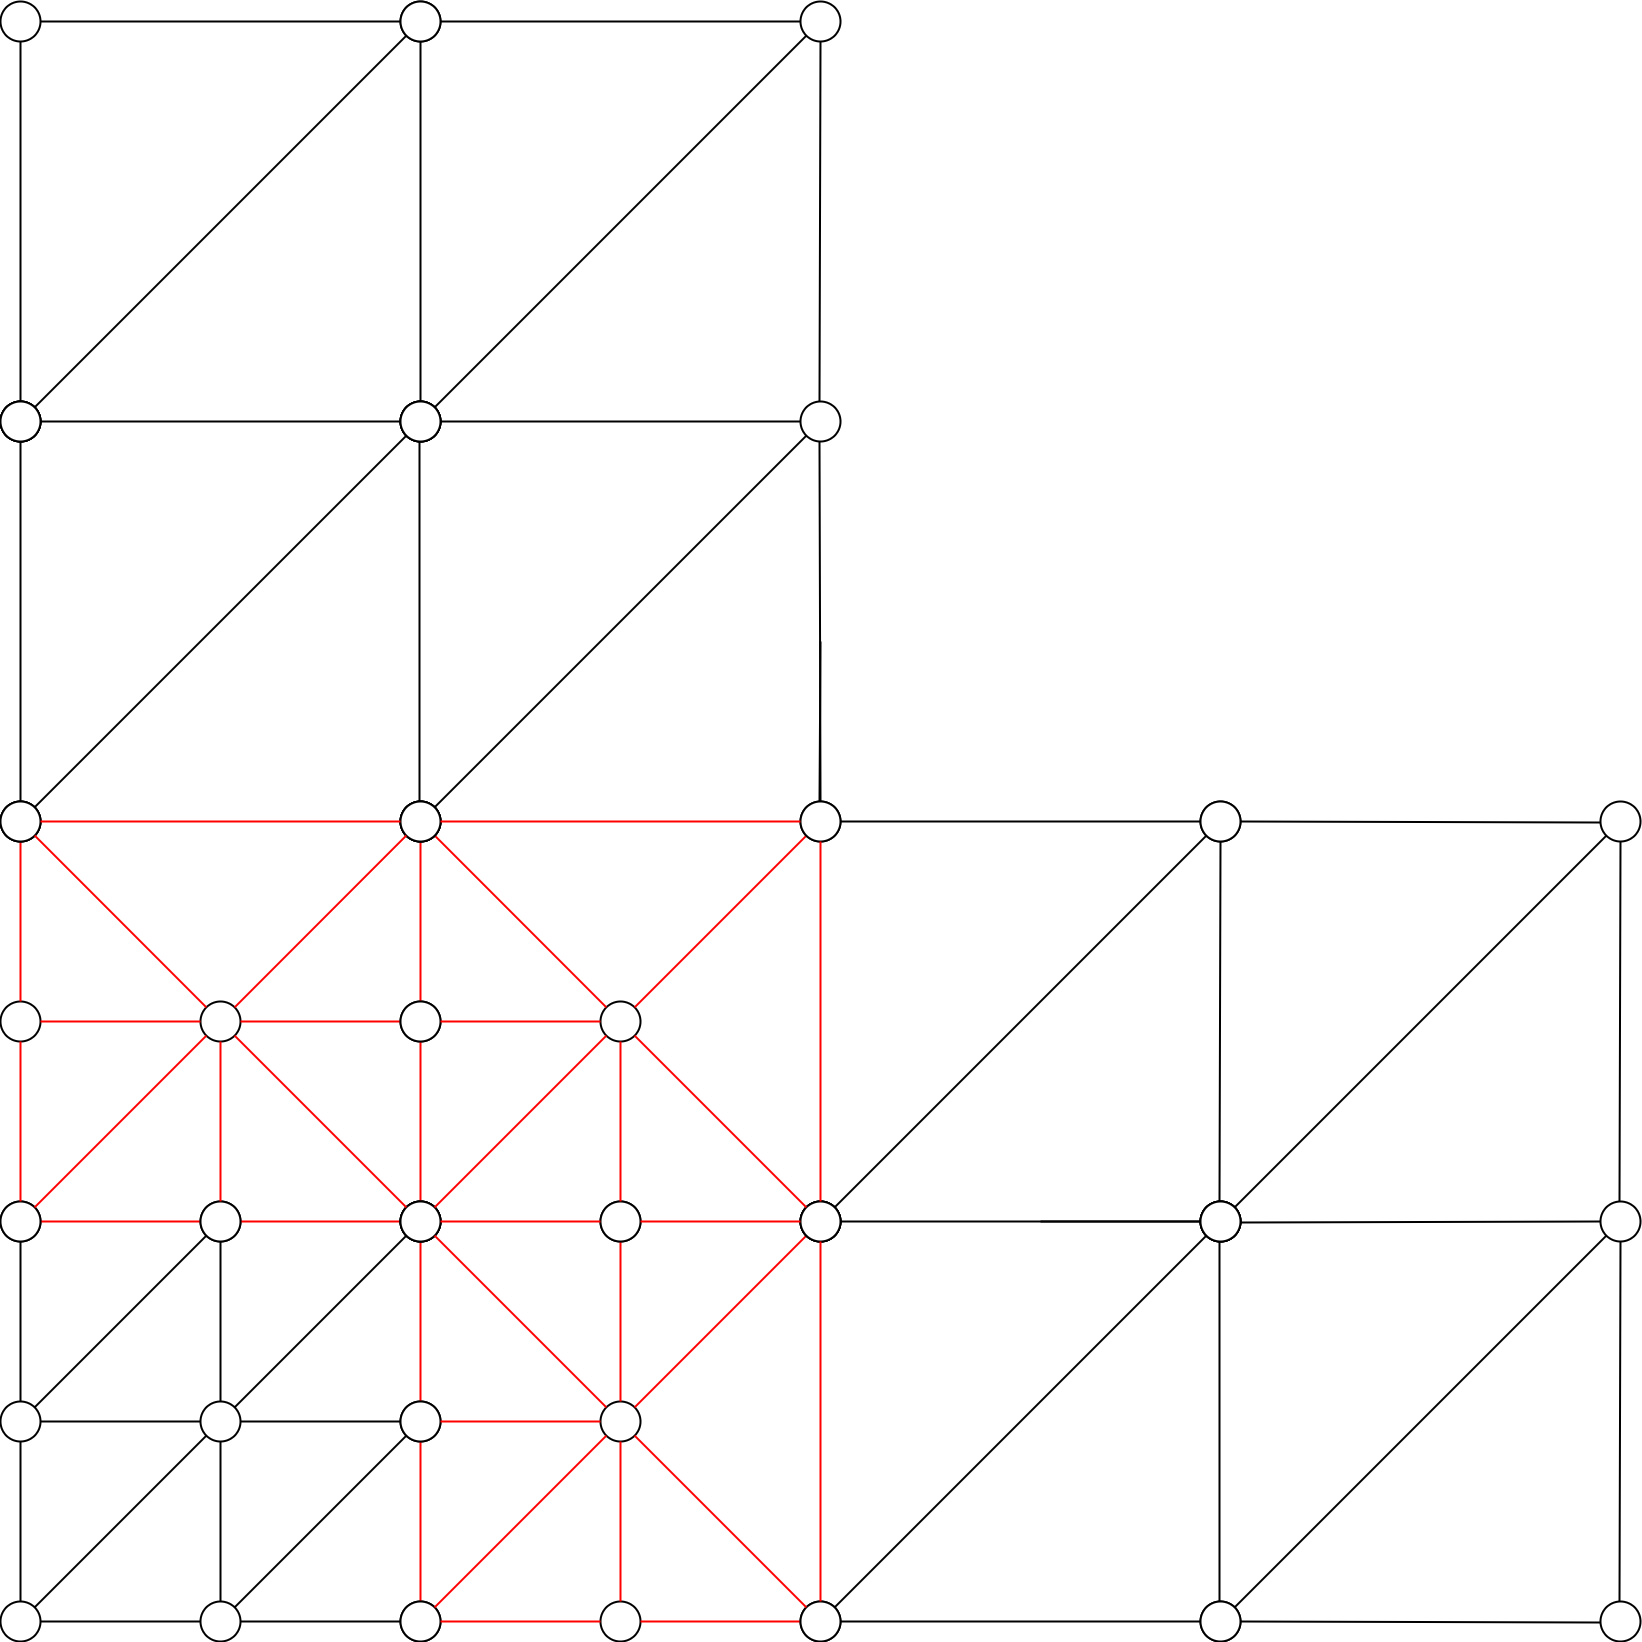
\includegraphics[width=0.45\textwidth]{geomipmapping-crack-avoidance-alternative-1} }}
  \qquad
  \subfloat[\centering Using only the top-most $2\times3$ subblocks and the right-most $3\times2$ subblocks for the triangle fans.]{{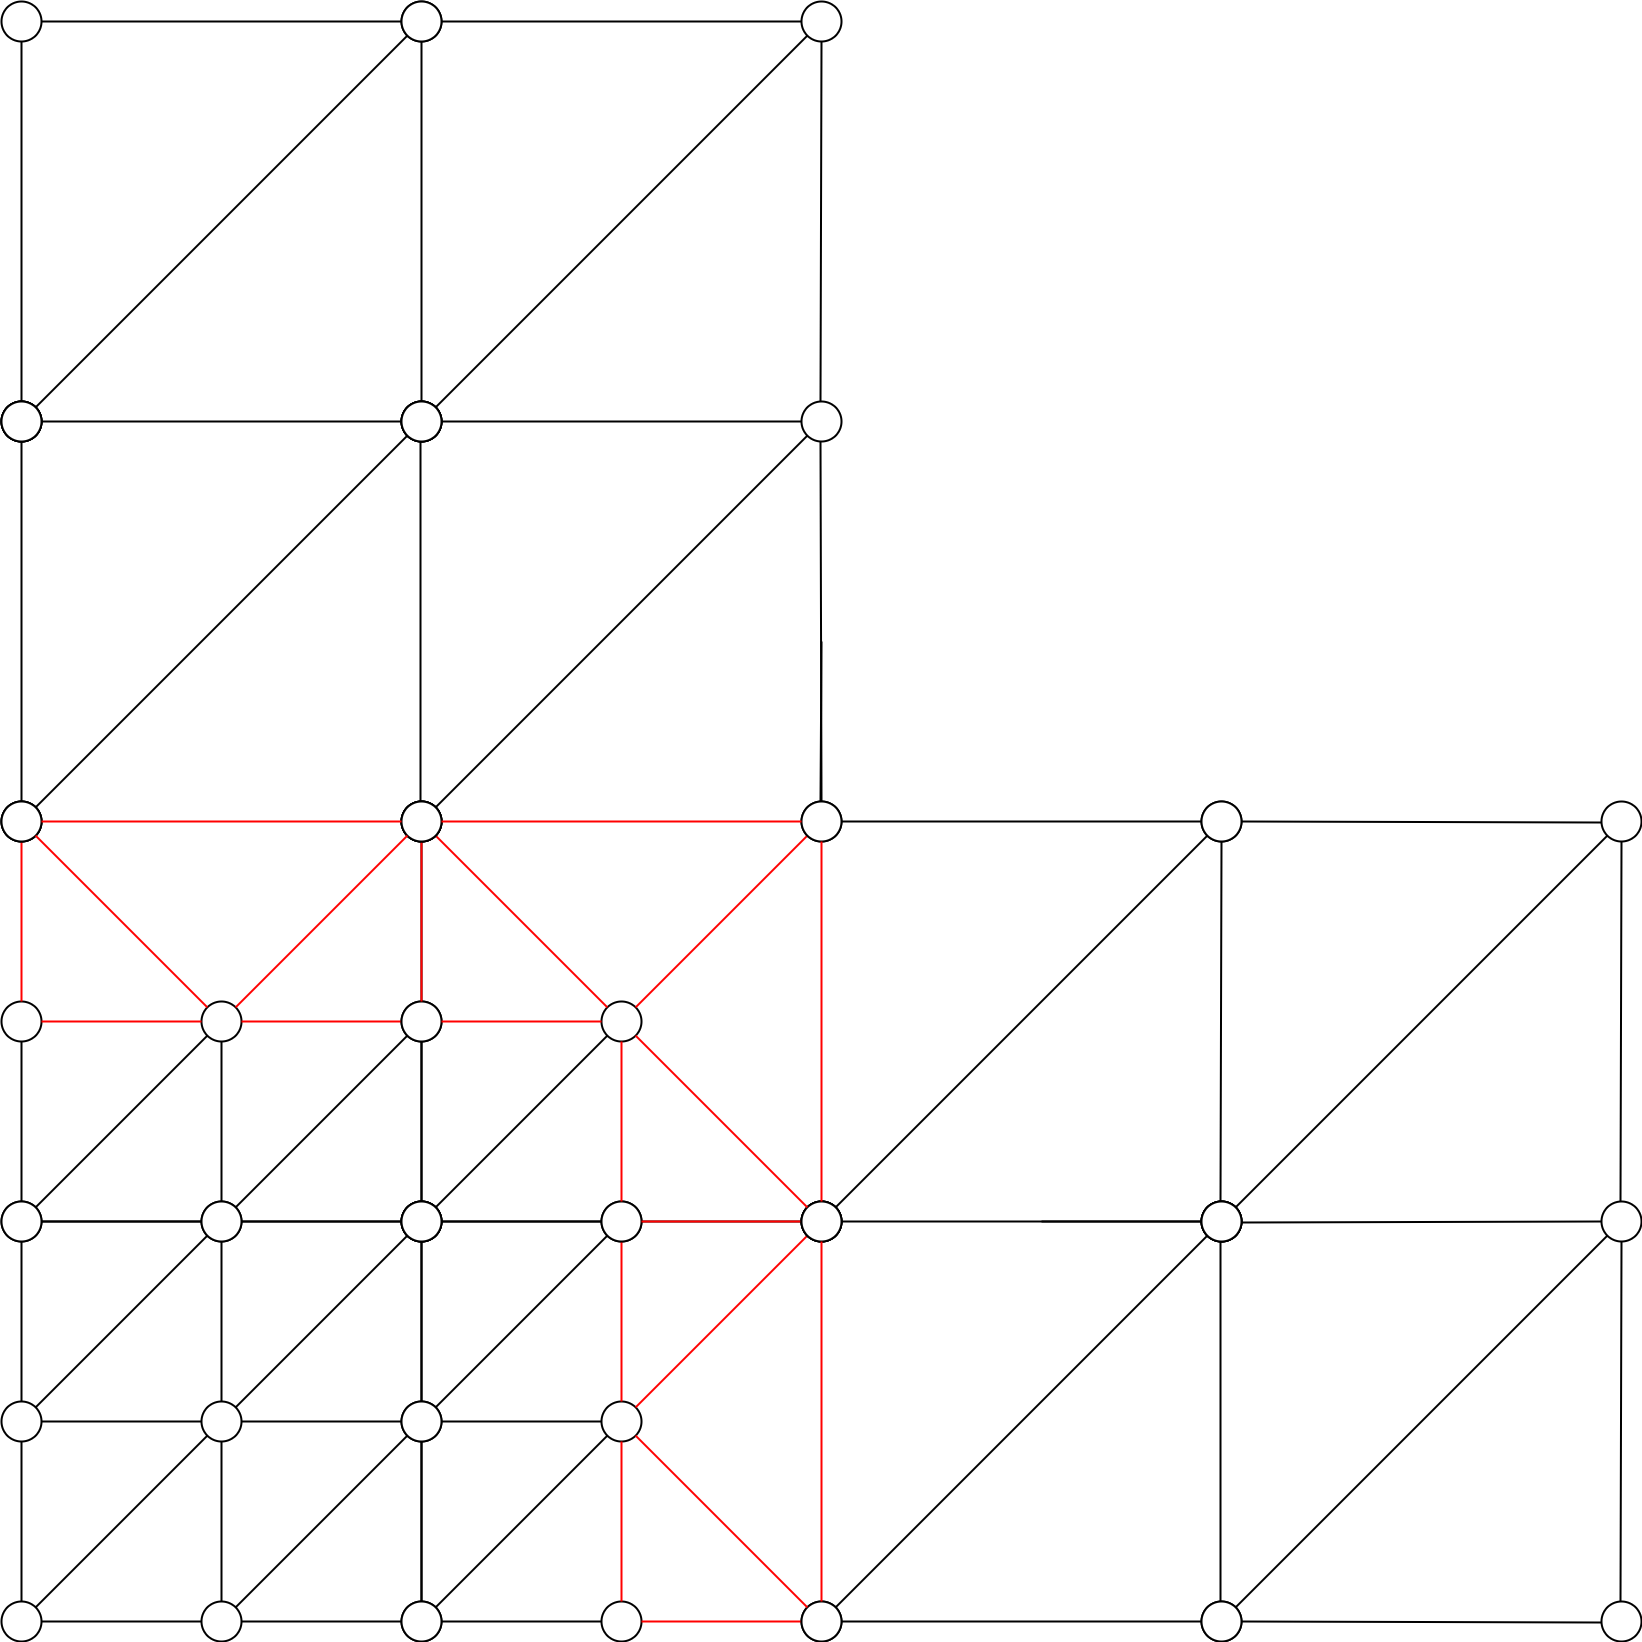
\includegraphics[width=0.45\textwidth]{geomipmapping-crack-avoidance-alternative-2} }}
  \caption{Two alternative triangle fan-based methods to avoid cracks between a LOD 2 and two LOD 1 GeoMipMaps of three $5 \times 5$ blocks. The border subblocks are marked in red.}\label{fig:geomipmapping-crack-avoidance-alternative}
\end{figure}

Regardless of the rendering approach, a neighborhood structure consisting of the LOD levels of the left, right, top and bottom 
neighboring blocks needs to be stored per block, so that the algorithm knows how to perform the vertex omission. The LOD levels of each block change continually each frame, which means 
that the neighborhood structure of each block also gets updated each frame.

\subsection{Other Optimizations}
\paragraph{Vertex Morphing}
GeoMipMapping can be extended with vertex morphing in order to decrease popping.




\section{Geometry Clipmaps}
Geometry Clipmaps is a terrain rendering technique published by Hoppe and Losasso in TODO.
The follow-up GPU-based 

%\section{CDLOD}
%TODO

\section{Concurrent Binary Trees}
TODO

\section{GPU Tessellation Shaders}


\chapter{Terrain LOD in Real-world Systems}
This chapter lists a selection of real-world examples of terrain LOD algorithms in use,
such as game engines and geographic information systems (GIS).
\section{Game Engines}
\subsection{Godot}
Godot is a cross-platform game engine written in C\#, C++ and its own scripting language GDScript.
Terrains are supported in form of extensions developed by community members, which can be installed and used in Godot projects by game developers.
One such extension is Terrain3D by Cory Petkovsek \cite{godotterrain3dgithub} 
written in C++ for Godot 4. The LOD approach used in this extension is based on 
geometry clipmaps by Hoppe and Losasso \cite{geomclipmaps}. % TODO Explain algo in high-level fashion
The concrete implementation
of the geometry clipmap mesh code was created by Mike J Savage \cite{geomclipmapssavage}. 
\subsection{Unity}
\subsection{Unreal Engine}
Unreal Engine is another cross-platform game engine written in C++ and features
an integrated terrain system (called the Landscape system).
The technical documentation of Unreal Engine 5 mentions utilising geomipmapping for 
handling LOD for landscapes \cite{unrealengine5doc}. Geomipmapping is a terrain LOD approach developed 
in 2000 by de Boer \cite{geomipmapping}. % TODO Explain algo in high-level fashion
\section{Geographic Information Systems}

\chapter{ATLOD: A Terrain Level of Detail (Renderer)}
This chapter describes \textit{ATLOD} (short for \textbf{A} \textbf{T}errain \textbf{L}evel \textbf{o}f \textbf{D}etail (Renderer)), the demo terrain rendering application.
The implemented algorithm is mainly based on GeoMipMapping, but also draws some inspiration from GPU-based Geometry Clipmaps and other algorithms,
notably in its effective usage of the GPU. 

\section{Preliminaries}
\subsection{Used Technologies}
ATLOD is written in C++17 and OpenGL 4.2.
For compiling build files, CMake (minimum version 3.5) is used.
ATLOD uses the following third-party libraries:
\begin{itemize}
  \item GLM: The \textit{OpenGL Mathematics (GLM)} library provides functionality for the mathematics of graphics programming, such as classes for vectors, matrices and perspective transformations.
  \item GLEW: The \textit{OpenGL Extension Wranger Library (GLEW)} is an extension loading library for OpenGL. 
  \item GLFW: \textit{GLFW} is a multi-platform library for desktop-based OpenGL applications, offering an API for managing windows, contexts and input handling.
  \item ImGui: \textit{Dear ImGui} is a multi-platform graphical user interface library developed by Omar Cornut TODO cite.
  \item STB: STB is a collection of header-only libraries developed by Sean Barrett TODO cite. ATLOD uses \texttt{stb\_image.h} for loading images of heightmaps and textures.
\end{itemize}

ATLOD was developed with Qt Creator 9.6.1. The source code is hosted on GitHub on the repository AmarTabakovic/3d-terrain-with-lod
and is licensed under TODO.

\section{Basic Setup and Architecture}
\subsection{Overview}
TODO High-level class diagram

\subsection{Shaders}
The class \texttt{Shader} encapsulates a shader program consisting of a vertex shader and a fragment shader.
It's based on the ``Shaders'' chapter in \textit{Learn OpenGL - Graphics Programming} \cite{learnopengl}.

\subsection{Camera}
The camera class is based on the ``Camera'' chapter in \textit{Learn OpenGL - Graphics Programming} \cite{learnopengl}.
The camera is defined by its yaw and pitch angles, which are used to construct the front, up and right 
camera vectors. The camera also consists of its position, of its near and far $z$-values, of its aspect ratio,
zoom, and of its flight and look-around velocities. The aspect ratio, near and far values and zoom are used to 

\subsubsection{Automatic Flying and Rotation}
ATLOD supports automatic flying of the camera using two given world-space coordinates.
The coordinates can be entered in a dialogue window and the flight velocity is adjustable with a slider.

The flying is implemented by linearly interpolating between the starting coordinate $\mathbf{p}_{start}$ 
and the end coordinate $\mathbf{p}_{end}$ with an interpolation factor $t$ in the main game loop.
More precisely, the direction is calculated by precomputing the direction vector $\mathbf{v}_{flyDir} = \mathbf{p}_{end} - \mathbf{p}_{start}$ and then by calculating
\begin{align*}
  \mathbf{p}_{new} = \mathbf{p}_{start} + t \cdot \mathbf{v}_{flyDir}.
\end{align*}
The interpolation factor $t$ starts at 0 and gets increased by a small value $0< t_{step}\leq1$ every frame until 
$t = 1$. This $t_{step}$ is adjustable by the user and corresponds to the previously mentioned flight velocity.

The class \texttt{Camera} contains a method \texttt{lerpFly()} which gets called each frame and performs the above calculation, as shown in listing \ref{lst:lerpfly}.
\begin{lstlisting}[
  language={C++},
  label={lst:lerpfly}
  caption={Method \texttt{Camera::lerpFly()} that linearly interpolates between $\mathbf{p}_{start}$ and $\mathbf{p}_{end}$.}]
void Camera::lerpFly(float lerpFactor)
{     
    _position = origin + direction * lerpFactor;
}
\end{lstlisting}

The main render loop contains the snippet shown in listing \ref{lst:mainloopcam}
\begin{lstlisting}[
  language={C++},
  label={lst:mainloopcam}
  caption={Snippet in the main render loop that is responsible for flying.}]
float posLerp = 0.0f;
// ...
void run() {
    while (!glfwWindowShouldClose(window)) {
        // ...
        if (camera.isFlying) {
            camera.lerpFly(posLerp);
            posLerp += 0.0005 + flightVel / 50000;

            if (posLerp >= 1.0f) {
                camera.isFlying = false;
                posLerp = 0.0f;
            }
        }
        // ...
    }
}
\end{lstlisting}

The automatic camera rotation works similarly, but interpolates from the initial yaw $yaw_{init}$ to
$yaw_{init} + 2\pi$ with
\begin{align*}
  yaw_{new} = yaw_{init} + t \cdot 2\pi. 
\end{align*}

\subsection{Skybox}
A \textit{skybox} is a box in world space that simulates the sky using
six texture images, one for each side of the box. 
Skyboxes are rendered with \textit{cubemaps}

The skybox implemented in ATLOD is based on the ``Cubemaps'' section in the ``Advanced OpenGL'' chapter in \textit{Learn OpenGL - Graphics Programming} \cite{learnopengl}.
It is encapsulated in the class \texttt{Skybox}.


An improvement over the current skybox would be to actually calculate the \textit{atmospheric scattering},
which would deliver a more realistic and flexible daytime-based lighting.
A suitable approach would be \textit{precomputed atmospheric scattering} by Bruneton and Neyret \cite{precomputedatmosphericscattering}.

\subsection{Base Terrain}
The base \texttt{Terrain} class is the superclass of all terrain LOD algorithms and 
contains fields that are common between different terrain LOD algorithms,
such as the heightmap, shader, width, height, and more.
It also contains the three virtual methods \texttt{loadBuffers}, \texttt{render()}
and \texttt{unloadBuffers()}, which all terrain subclasses must implement.

The base terrain is structured as shown in listing TODO.

\subsection{Heightmaps}
The class \texttt{Heightmap} represents a heightmap and its data.
Like many game engines today, such as Unity and Unreal Engine, ATLOD supports heightmaps as 16-bit grayscale PNG images, which allow for 
strorage of up to $2^{16}-1=65535$ height values per pixel. 

\subsubsection{Heightmap Preprocessing}
Digital elevation model (DEM) data is commonly offered in the GeoTIFF file format by various DEM providers,
such as SwissTopo and OpenTopography.
GeoTIFF files can be converted into PNG using GIS software, such as 
QGIS or GDAL. 

A small Python 3 command line utility named \texttt{geotiff-to-png} for converting GeoTIFF files into 16-bit grayscale PNG images
is available in the repository of ATLOD in the \texttt{scripts} folder. 

\subsubsection{Loading}
The method \texttt{load()} is responsible for loading a heightmap
located at a given file path \texttt{fileName}.
Depending on the file extension of \texttt{fileName}, 
TODO.

The height values are stored in the field \texttt{\_data} of type \texttt{std::vector<unsigned short>}.

For terrain LOD algorithms using heightmap displacement inside the vertex shader, 
the \texttt{load()} method offers the possibility to optionally load the heightmap 
directly into an OpenGL texture object. The ID is stored on the current \texttt{Heightmap}
instance in the field \texttt{\_heightmapTextureId}, so that multiple different 
\texttt{Terrain} instances can share the same heightmap if needed.

\section{Naive Brute-force Algorithm}
The naive brute-force algorithm, which simply renders every vertex without any LOD considerations, is encapsulated in the class \texttt{NaiveRenderer}.

\subsection{Vertex and Index Organisation}
A vertex consists of its $(x,y,z)$-position,
its normal vector $(n_x,n_y,n_z)$ and of its
texture coordinates $(u,v)$. All components
are 4-byte floating point values, which means that 
per vertex, $4 \times 8 = 32$ bytes of GPU memory
get allocated. These attributes are organized 
in a vertex array object stored in the field \texttt{\_vao}.

The indices are organized such that they can be rendered as triangle strips with \texttt{GL\_TRIANGLE\_STRIPS}.
Each row is separated using a special marker index named \texttt{RESTART}, which is set to the maximum possible \texttt{GLuint} value and is used for the \texttt{GL\_PRIMITIVE\_RESTART} mode,
allowing for the entire terrain to be rendered in a single \texttt{glDrawElements()} call. This draw call happens every frame in the 
method \texttt{render()}. Figure~\ref{fig:naive-triangles} shows the organization of indices for rendering the terrain as triangle strips.

\begin{figure}[H]
  \centering
  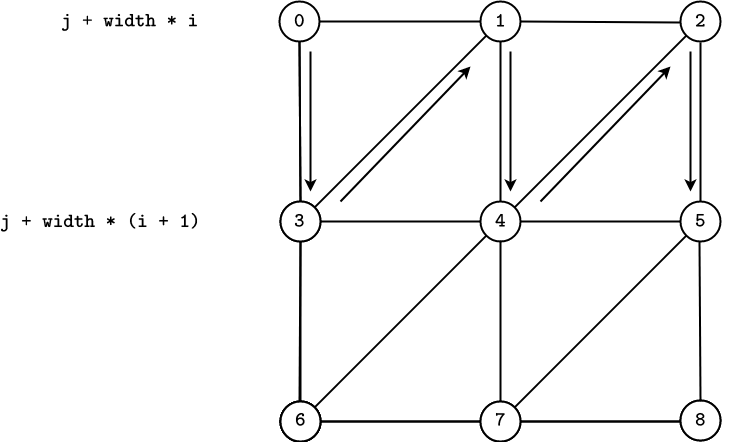
\includegraphics[width=0.9\textwidth]{atlod-naive-triangles}
  \caption{Example of a terrain layout for triangle strips. The looping index \texttt{i} goes from 0 to the terrain height and \texttt{j} from 0 to the terrain width. The final indices to be rendered are 0,3,1,4,2,5,\texttt{RESTART},3,6,4,7,5,8,\texttt{RESTART}.}\label{fig:naive-triangles}
\end{figure}

\subsubsection{Loading}
The method \texttt{loadBuffers()} is responsible for loading the data into the vertex and index buffer.
The first step is the generation of the normal vectors. This is done in the method \texttt{loadNormals},
where the normals of each vertex are calculated into an intermediate vector \texttt{\_normals}.

The normals are calculated as follows. Each vertex consists 
of its $\mathbf{p}_{pos} = (x,y,z)$ position, where the $(x,z)$-coordinates
are given by the current position relative to the heightmap size and the $y$-coordinate is retrieved from the heightmap in memory.
The four orhogonally neighboring points 

Geometrically, the direction of a sum of vectors is given by 
constructing a chain of these vectors, such that the 
beginning of the next vector is at the tip of the previous vector,
and then ``walking'' along all vectors from the first to the last vector.

\subsection{Shading}
The shading is calculated with the Phong shading technique in the fragment shader.

\section{GeoMipMapping}
The implementation supports most basic functionalities described in the original paper, but differs in a few key aspects.
It also draws some inspiration from other approaches, most notably from GPU-based Geometry Clipmaps by Hoppe and Asirvatham
and from ``Terrain Rendering in Frostbite Using Procedural Shader Splatting'' by Andersson for the Frostbite game engine TODO cite.
Both approaches utilize a single flat mesh (positioned around the viewer in Hoppe and Asirvatham's approach) and store the heightmap as a texture object. The height values are sampled in the vertex shader, which are then 
used to displace the flat mesh on the $y$-axis. 

The idea of using a texture object for the heightmap is applied to ATLOD's GeoMipMapping implementation.
Rather than generating vertex buffers for each block and loading in the height values into the vertices directly (as in the naive renderer implementation),
a single flat mesh with the side length of the block size is generated once at load time. At render time, for each block the mesh is translated 
to the block's world-space position and the height values get sampled from the heightmap, which is stored as a texture object.
The upcoming subsections describe the approach in greater detail.

\subsection{Block Structure}
As described in the high-level overview of the GeoMipMapping algorithm, 
the algorithm splits up the terrain into square blocks of side length $2^n+1$.

In this implementation, a block is the structure containing information of a
particular section of the terrain. The class \texttt{GeoMipMappingBlock}
represents such a block and contains the following fields:
\begin{itemize}
  \item \texttt{unsigned \_blockId}: this field stores the ID of the current block.
  \item \texttt{unsigned \_currentBorderBitmap}: this field stores the current border permutation as a bitmap.
  \item \texttt{float \_minY} and \texttt{float \_maxY}: these two fields store the minimum and maximum $y$-coordinates of that particular block.
  \item \texttt{glm::vec2 \_translation}: this field stores the 2-dimensional translation vector for translating the flat mesh to the block's actual position.
  \item \texttt{glm::vec3 \_aabbCenter} and \texttt{glm::vec3 \_trueCenter}: \texttt{\_aabbCenter} stores the position of the center of the AABB of the block, i.e. its $y$-coordinate is set to $\texttt{\_maxY} - \texttt{\_minY}$.
        This field is used for view-frustum culling during rendering.
        The field \texttt{\_trueCenter} on the other hand stores the actual center position of that block in world-space, i.e. its $y$-coordinate is computed from the heightmap. 
        This field is used for the distance calculation for the LOD determination during rendering.
\end{itemize}

\subsection{Vertex and Index Organisation}
ATLOD's GeoMipMapping implementation consists of a single vertex buffer and index buffer.
The vertex buffer contains the vertices for a single flat $b \times b$ mesh centered around $(0,0,0)$, where $b = 2^n + 1$ is the block size and $n$ is the maximum LOD level.
The vertices of the flat mesh only consist of 4-byte floating point $(x,z)$-coordinates, since the mesh is flat.

The index buffer contains the 4-byte unsigned integer indices of the flat mesh and is organized as follows:
the flat mesh is split up into its border area and center area.
The reason for splitting the mesh up this way will be made clear shortly.
The first part of the index buffer stores the indices of the border area
for every LOD level and border permutation, and
the second part of the index buffer stores the center area for every LOD level. 
What a \textit{border permutation} is will be explain in the next section.
Figure \ref{fig:atlod-geomipmapping-index-buffers} shows the described index buffer 
organisation.

\begin{figure}[H]
  \centering
  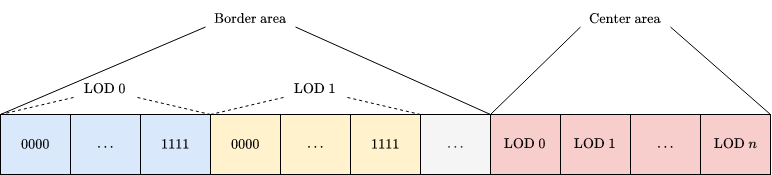
\includegraphics[width=1.0\textwidth]{atlod-geomipmapping-index-buffer.png}
  \caption{The index buffer organisation of the single flat block. The variable $n$ corresponds to the maximum LOD level.}\label{fig:atlod-geomipmapping-index-buffers}
\end{figure}

\subsubsection{Border Permutations}
A border permutation is defined to be a 4-tuple $(t,b,l,r)$,
where $t,b,l,r$ correspond to top, bottom, left and right, and where each entry is set to 1 if the block on 
the corresponding side has a lower LOD, and 0 otherwise. For example, if the top and right neighboring blocks
have a lower LOD than the current block, the border permutation is $(1,0,0,1)$.
These border permutations can also be expressed as bitfields, e.g. \texttt{1001},
which allows for easy indexing into the subset of the index buffer containing the relevant indices.
The number of possible permutations is $2^4=16$.
In order for this approach to work, the difference in LOD level between any two bordering blocks 
must be at most 1. 
A similar approach is described by Andersson in SIGGRAPH 2007 for the terrain rendering 
in the Frostbite game engine for the game Battlefield 2, with their approach requiring only 9 permutations.
Figure \ref{fig:atlod-geomipmapping-crack-avoidance} shows all possible border permutations of a $5 \times 5$ block at LOD level 2.

\begin{figure}[H]
  \centering
  \subfloat[\centering \texttt{0000}.]{{
\includegraphics[width=0.17\textwidth]{atlod-geomipmapping-0000.png} }}
  \qquad
  \subfloat[\centering \texttt{0001}.]{{
\includegraphics[width=0.17\textwidth]{atlod-geomipmapping-0001.png} }}
  \qquad
  \subfloat[\centering \texttt{0010}.]{{
\includegraphics[width=0.17\textwidth]{atlod-geomipmapping-0010.png} }}
  \qquad
  \subfloat[\centering \texttt{0011}.]{{
\includegraphics[width=0.17\textwidth]{atlod-geomipmapping-0011.png} }}

  \subfloat[\centering \texttt{0100}.]{{
\includegraphics[width=0.17\textwidth]{atlod-geomipmapping-0100.png} }}
  \qquad
  \subfloat[\centering \texttt{0101}.]{{
\includegraphics[width=0.17\textwidth]{atlod-geomipmapping-0101.png} }}
  \qquad
  \subfloat[\centering \texttt{0110}.]{{
\includegraphics[width=0.17\textwidth]{atlod-geomipmapping-0110.png} }}
  \qquad
  \subfloat[\centering \texttt{0111}.]{{
\includegraphics[width=0.17\textwidth]{atlod-geomipmapping-0111.png} }}

  \subfloat[\centering \texttt{1000}.]{{
\includegraphics[width=0.17\textwidth]{atlod-geomipmapping-1000.png} }}
  \qquad
  \subfloat[\centering \texttt{1001}.]{{
\includegraphics[width=0.17\textwidth]{atlod-geomipmapping-1001.png} }}
  \qquad
  \subfloat[\centering \texttt{1010}.]{{
\includegraphics[width=0.17\textwidth]{atlod-geomipmapping-1010.png} }}
  \qquad
  \subfloat[\centering \texttt{1011}.]{{
\includegraphics[width=0.17\textwidth]{atlod-geomipmapping-1011.png} }}

  \subfloat[\centering \texttt{1100}.]{{
\includegraphics[width=0.17\textwidth]{atlod-geomipmapping-1100.png} }}
  \qquad
  \subfloat[\centering \texttt{1101}.]{{
\includegraphics[width=0.17\textwidth]{atlod-geomipmapping-1101.png} }}
  \qquad
  \subfloat[\centering \texttt{1110}.]{{
\includegraphics[width=0.17\textwidth]{atlod-geomipmapping-1110.png} }}
  \qquad
  \subfloat[\centering \texttt{1111}.]{{
\includegraphics[width=0.17\textwidth]{atlod-geomipmapping-1111.png} }}
  \caption{Every possible border permutation for a LOD 2 GeoMipMap of a $5 \times 5$ block. The center subblocks have been omitted from the illustration.}\label{fig:atlod-geomipmapping-crack-avoidance}
\end{figure}

This makes clear why the flat mesh is split into its border and center area.
The center area only depends on the LOD level and is the same 
regardless of the current border permutation. 
Not splitting the flat mesh up into its border and center area 
would require longer index buffer generation times and consume 
significantly more GPU memory.

\subsubsection{Starts and Sizes Lists}
The organisation of the index buffer as presented requires some additional
management of the start indices and sizes of the subsets of the index buffer. The \texttt{GeoMipMapping} class 
contains four members of the type \texttt{std::vector<unsigned>}:
\texttt{\_borderStarts}, \texttt{\_borderSizes}, \texttt{\_centerStarts} and \texttt{\_centerSizes}.
The \texttt{\_borderStarts} and \texttt{\_borderSizes} lists store the starting index 
(into the index buffer) and 
the number of indices, for a subset of the index buffer containing the indices of the border area for a given border permutation and LOD level.
Both the lists are indexed by multiplying the current LOD level by 16 
and then adding the current border permutation to it.
The \texttt{\_centerStarts} and \texttt{\_centerSizes} lists are indexed similarly,
except that they are indexed simply with the current LOD level.

In order to illustrate the idea more clearly, the following example is given:
say that the current block has a LOD level of 1 and every neighboring block has the 
same LOD level (i.e. the border permutation is $(0,0,0,0)$). 
We want to render the block, which means 
we need to retrieve the indices for the flat mesh 
at the LOD level 1 and for the border permutation \texttt{0000}.
The start index and the size for the border area are retrieved with \texttt{\_borderStarts[1 * 16 + 0b0000]}
and \texttt{\_borderSizes[1 * 16 + 0b0000]} respectively, and for 
the center area with \texttt{\_centerStarts[1]} and \texttt{\_centerSizes[1]}.
These four values are passed to the two \texttt{glDrawElements()} draw calls for the block,
which renders the flat mesh at the chosen LOD level 1 and border permutation $(0,0,0,0)$.
The full rendering process is described in the subsection ``Rendering'' of this section.
Figure \ref{fig:atlod-starts-sizes-example} illustrates this example.

\begin{figure}[H]
  \centering
  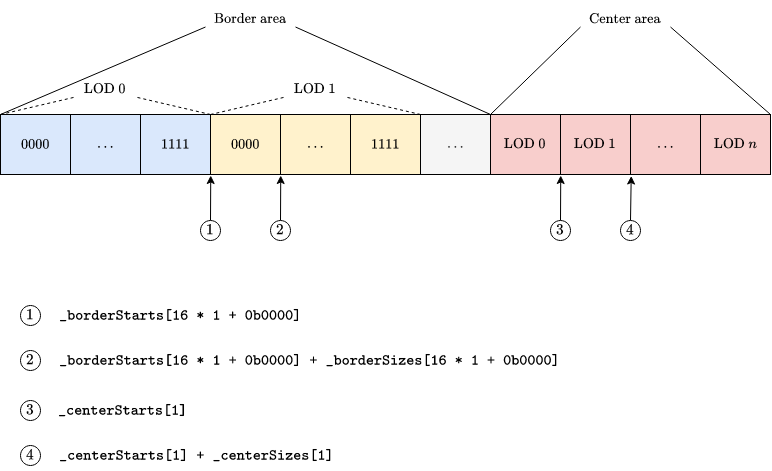
\includegraphics[width=1.0\textwidth]{atlod-starts-sizes-example.png}
  \caption{Illustration of accessing the start index and size of the subsets of the index buffer for LOD 1 and border permutation $(0,0,0,0)$}\label{fig:atlod-starts-sizes-example}
\end{figure}

\subsubsection{Loading}
Now that the organisation of the vertices and indices 
has been presented, the loading mechanisms are described.
The vertex and index buffers get loaded in the method \texttt{loadBuffers()},
which calls the two helper methods \texttt{loadVertices()} an \texttt{loadIndices()}.

The method \texttt{loadVertices()} simply generates the vertex array object with its ID stored in the field \texttt{\_vao}
and loads the vertices of the flat mesh of size $blockSize \times blockSize$
centered around $(0,0,0)$ into a vertex buffer with its ID stored in the field \texttt{\_vbo}.
\begin{lstlisting}[
  language=C++,
  caption={Method \texttt{GeoMipMapping::loadVertices()} that generates the vertex array object and loads the
  vertex buffer with the flat mesh of size $blockSize \times blockSize$ centered around $(0,0,0)$.}]
void GeoMipMapping::loadVertices()
{
    for (int i = 0; i < _blockSize; i++) {
        for (int j = 0; j < _blockSize; j++) {
            // Load vertices around center point 
            float x = (-(float)_blockSize / 2.0f + (float)_blockSize * j / (float)_blockSize);
            float z = (-(float)_blockSize / 2.0f + (float)_blockSize * i / (float)_blockSize);

            _vertices.push_back(x); // Position x 
            _vertices.push_back(z); / Position z 
        }
    }

    glGenVertexArrays(1, &_vao);
    glBindVertexArray(_vao);

    glGenBuffers(1, &_vbo);
    glBindBuffer(GL_ARRAY_BUFFER, _vbo);
    glBufferData(GL_ARRAY_BUFFER, _vertices.size() * sizeof(float), &_vertices[0], GL_STATIC_DRAW);

    // Position attribute
    glVertexAttribPointer(0, 2, GL_FLOAT, GL_FALSE, 2 * sizeof(float), (void*)0);
    glEnableVertexAttribArray(0);
}
\end{lstlisting}

The index loading mechanism is more complex.
The top-level index loading method \texttt{loadIndices()}
performs the following operations:
\begin{itemize}
  \item It loads the LOD 0 and LOD 1 representation of the flat mesh using \texttt{loadLod0()} and \texttt{loadLod1()} respectively. The LOD 0 and LOD 1 indices require special treatment. They are stored as borders and do not have a center.
  \item It loads the rest of the indices from LOD 2 to the maximum LOD level, by first loading in the border indices with \texttt{loadBorderAreaForLod()}
        and then the center areas with \texttt{loadCenterAreaForLod()}.
\end{itemize}

\subsection{LOD Selection}
The LOD of ATLOD's GeoMipMapping implementation is based on the Euclidean distance $dist$ between 
the camera's position $\mathbf{p}_{camPos} = (camPos_x, camPos_y, camPos_z)$ 
and the block's center point $\mathbf{p}_{blockCenter} = (blockCenter_x, blockCenter_y, blockCenter_z)$
\begin{align*}
  dist = \sqrt{ \begin{aligned} & (blockCenter_x - camPos_x)^2 + (blockCenter_y - camPos_y)^2 \\
          & + (blockCenter_z-camPos_z)^2 \end{aligned}}.
\end{align*}
A minor optimization for this calculation is possible by instead calculating the LOD using the squared distance, 
which avoids an expensive square-root call.

Two different LOD determination modes are possible: the \textit{linearly growing distance} and the \textit{exponentially growing distance}.
Both use a base distance value $baseDist$ which 
can be set by the user. Note that $baseDist$ should be larger than $blockSize$,
as otherwise cracks in the terrain may occur, but also not too large, 
so that the performance is still adequate.
The LOD computed by the linearly growing distance can be defined with the following recursive formula
\begin{align*}
  lod_{lin}(dist, i) = 
  \begin{cases}
    l - i  + 1& dist \leq i \cdot baseDist\\
    lod_{lin}(dist, i + 1) & i \cdot baseDist < dist < (l + 1) \cdot baseDist\\
    0 & \text{otherwise}
  \end{cases},
\end{align*}
where $i$ starts at 1 and $l$ is the maximum LOD level.
As a basic example, say that $l=3,baseDist=100,dist=250$.
We begin computing the LOD level with $lod_{lin}(250,1)$.
The second condition $1 \cdot 100 < 250 < 4 \cdot 100$ holds, so we continue with $lod_{lin}(250,2)$.
Again, the second condition $2 \cdot 100 < 250 < 4 \cdot 100$ holds, so we continue with $lod_{lin}(250,3)$.
Now, the first condition $250 \leq 3 \cdot 100$ holds, so the entire expression evaluates to $3-3+1=1$,
which means we set the LOD level of the block to 1.

The exponentially growing distance is defined very similarly:
\begin{align*}
  lod_{exp}(dist, i) = 
  \begin{cases}
    l - i + 1 & dist \leq i \cdot baseDist\\
    lod_{exp}(dist, 2i) & i \cdot baseDist < dist < (l+1) \cdot baseDist\\
    0 & \text{otherwise}
  \end{cases}.
\end{align*}

The above expressions are implemented in the \texttt{GeoMipMapping} class in a single method \texttt{determineLodDistance()}.
The LOD determination mode can be set with the boolean argument \texttt{doubleEachLevel}.
Additionally, the minimum and maximum LOD levels can be manually set to be different from 0 and $l$ respectively 
by the user, with the fields \texttt{\_minLod} and \texttt{\_maxLod}. 
Note that the user defined \texttt{\_minLod} and \texttt{\_maxLod} values
are both set to $\max\{0,\texttt{\_minLod}\}$ and $\min\{l,\texttt{\_maxLod}\}$ respectively in the constructor, 
so that the LOD level does not go out of bounds.
Listing \ref{lst:determineloddistance} shows the method \texttt{determineLodDistance}.

\begin{lstlisting}[
  language={C++},
  label={lst:determineloddistance},
  caption={Method \texttt{GeoMipMapping::determineLodDistance()} that determines the LOD level of a block 
  based on its distance to the camera.}]
unsigned GeoMipMapping::determineLodDistance(float squareDistance, float baseDist, bool doubleEachLevel)
{
    unsigned distancePower = 1;
    for (unsigned i = 0; i < _maxLod - _minLod; i++) {
        if (squaredDistance < distancePower * distancePower * baseDist * baseDist)
            return _maxLod - i;

        if (doubleEachLevel)
            distancePower <<= 1;
        else
            distancePower++;
    }
    return _minLod;
}
\end{lstlisting}

Figure \ref{fig:atlod-lin-exp} shows both LOD determination modes in action.
\begin{figure}[H]
  \centering
  \subfloat[\centering Linearly growing distance mode.]{{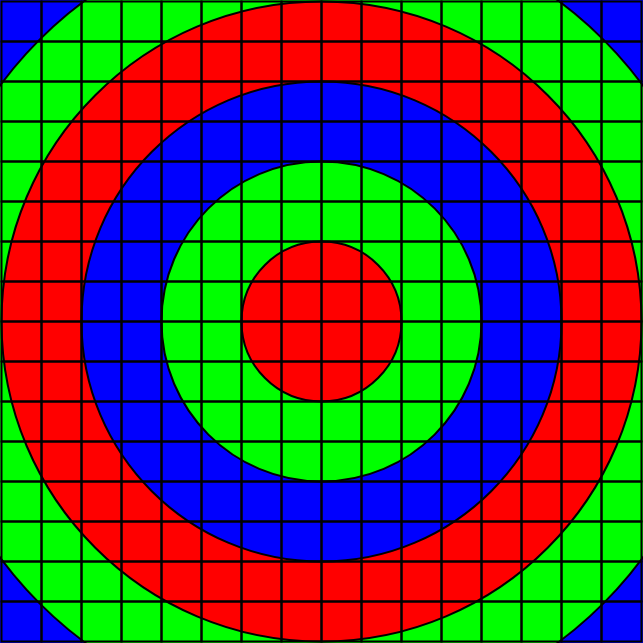
\includegraphics[width=0.4\textwidth]{atlod-lod-linear} }}
  \qquad
  \subfloat[\centering Exponentially growing distance mode.]{{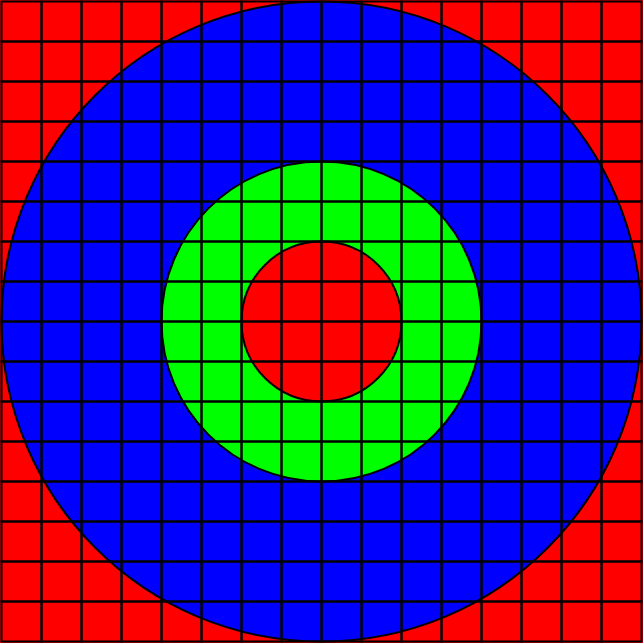
\includegraphics[width=0.4\textwidth]{atlod-lod-exponential} }}%
  \caption{Illustration of a flat terrain showcasing the linearly growing distance mode (a) and exponentially growing distance mode (b). The red, green and blue colors indicate successively lower LOD levels, starting from the maximum level in the center.}\label{fig:atlod-lin-exp}
\end{figure}

\subsection{View-frustum Culling}
View-frustum culling is implemented with the methods TODO in the \texttt{Camera} class.


\subsection{Rendering}
The method \texttt{render()} that is called each frame performs in two phases:
\begin{itemize}
  \item The first phase iterates through every block, calculates the distance between 
        the block's \texttt{\_trueCenter} and the camera's position, and updates the LOD level of the block 
        accordingly. 
  \item The second phase consists of performing view-frustum culling, setting the uniform variables in the shader,
        and finally rendering the block.
\end{itemize}

\subsubsection{Vertex Shader}
The vertex shader first translates the vertex from its initial position around $(0,0,0)$ to its actual world-space 
position using the uniform \texttt{vec2} variable \texttt{translation}.

\subsubsection{Fragment Shader}
The fragment shader 

The Phong shading is based on TODO cite and is performed with the following steps: 
first, the heightmap is sampled at the four orthogonally neighboring points $\mathbf{p}_{1,0} = (x + 1,z)$, $\mathbf{p}_{-1,0} = (x - 1,z)$, $\mathbf{p}_{0,1} = (x, z + 1)$ and $\mathbf{p}_{0,-1} = (x, z - 1)$,
where $(x,z)$ is the current texture coordinate for sampling the current height from the heightmap.
Using these four points, the slope in $x$ and $z$-direction can be calculated by computing
\begin{align*}
  dx = \mathbf{p}_{-1,0} - \mathbf{p}_{1,0}\\
  dz = \mathbf{p}_{0,-1} - \mathbf{p}_{0,1}.
\end{align*}
These values can now be used to create a normal vector
\begin{align*}
  \mathbf{n} = \frac{(dx, 2, dz)}{\lVert(dx,2,dz)\rVert}.
\end{align*}

Listing TODO shows the calculation of the normal vector from the heightmap texture.


\subsection{Conclusion}
The implementation still has some room for improvements, such as instanced rendering, geomorphing 
and a quadtree-based frustum culling. The memory consumption by the index buffer could be 
further brought down by only defining indices for the border permutations $(0,0,0,0),
(1,1,1,1),(1,1,0,0),(1,0,1,0),$$(1,1,1,0)$ and 
by rotating the mesh about the $y$-axis such that the borders align without cracks.

\chapter{Results}
A comparison with existing game engines is difficult. ATLOD is 
developed specifically and exclusively for terrain rendering, whilst game engines
contain other components and often perform various tasks in the background, which hinders an accurate performance comparison.

\section{Experimental Setup}
\subsection{Computer}
The computer used is a MacBook Air 2020 with an Intel CPU.
The specifications are displayed in table \ref{tbl:specs}:

\begin{table}[H]
  \begin{center}
    \begin{tabular}{ c|c }
      CPU & 1.1 GHz Dual-Core Intel Core i3\\
      \hline
      Memory & 8 GB 3733 MHz LPDDR4X\\
      \hline
      Graphics & Intel Iris Plus Graphics 1536 MB\\
      \hline
      OS & macOS Monterey Version 12.6
    \end{tabular}
  \end{center}
  \caption{The specifications of the used MacBook Air 2020.}\label{tbl:specs}
  \end{table}

\subsection{Height Data and GeoMipMapping Configuration}
The height data used is the SRTM 30m data set retrieved from OpenTopography TODO cite and covers 
a large extent of Switzerland (excluding the Grisons) and small parts 
of Germany, France and Italy. The total area is 130 km$^2$.
The heightmap file
is a $13922 \times 14140$ 16-bit greyscale PNG image converted 
from a GeoTIFF file, as shown in figure \ref{fig:results-heightmap}.

\begin{figure}[H]
  \centering
  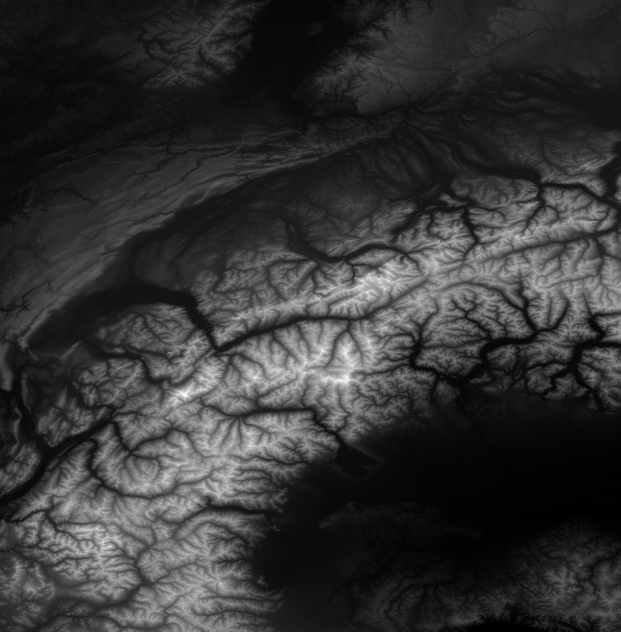
\includegraphics[width=0.7\textwidth]{results-heightmap}
  \caption{The $13922 \times 14140$ 16-bit greyscale heightmap used for benchmarking (retrieved from OpenTopography TODO cite). In this figure, the gray values were converted from 0,\dots,65535 to 0,\dots,255 in order to make the heights more visible.}\label{fig:results-heightmap}
\end{figure}

The GeoMipMapping algorithm is configured for the best balance between 
performance and visual accuracy as follows:
\begin{itemize}
  \item Block size: 257
  \item Fog: 0.003
  \item Minimum LOD: 0
  \item Maximum LOD: 8
  \item Base distance: 700
  \item LOD determination mode: Exponentially growing distance
\end{itemize}

\subsection{Benchmarks}
Two kinds of benchmarks are performed:
\begin{itemize}
  \item The first benchmark measures the performance, which measures the average FPS during rendering.
  \item The second benchmark measures the visual accuracy, i.e. the image difference between the ground truth (actual full-resolution terrain)
        and the terrain rendered with LOD.
\end{itemize}
For each of the benchmarks, two kinds of scenarios are performed:
\begin{itemize}
  \item The first scenario is the flyover from the bottom-left corner to the top-right, whilst the camera is looking down a certain angle.
        The $y$-coordinate and the front vector of the camera are fixed during this flyover.
  \item The second scenario is the $360^{\circ}$ rotation while stationary. 
\end{itemize}

\section{Performance}
\subsection{Flyover from Corner to Corner}
\subsection{360\textdegree~Rotation}

\section{Acurracy}
\subsection{Flyover from Corner to Corner}
\subsection{360\textdegree~Rotation}

\section{Theoretical Memory Consumption}
\subsection{RAM}


\subsection{GPU Memory}
While there is some complexity overhead in managing the index buffer 
in the presented way, the GPU memory usage is quite low.
The main bottleneck of this implementation in terms of GPU memory is 
the heightmap texture, which takes up 2 bytes per height value.
A solution would be to support 1-byte grayscale heightmaps. However, this would 
limit the number of possible height values to 256 and therefore produce
``blocky'' looking terrain.

On the other hand, memory consumption by the vertices and indices is quite low.
The number of vertices that are loaded on the GPU is only $b \times b$.

Table TODO shows memory usage by the heightmap texture, the vertex buffer and the index buffer 
with certain terrain sizes and block sizes.

% For example, for a block size of $2^8 + 1= 257$, the total number of vertices on the GPU is given by $257 \times 257 = 66049$, and the number of indices (manually calculated at load time) is 255086. 
% Assuming 4-byte floats for the $(x,z)$-vertices and 4-byte unsigned integers for the indices,
% the total memory taken up by the vertex and index buffer would be $66049 \times 2 \times 4 + 255086 \times 4 = 1548736 \text{ bytes}$, or 1.54 megabytes.

\chapter{Discussion}
Overall, the implemented algorithm works decently well, despite 
lacking some features for it to be fully optimized.
The configurability of the implementation allows for usage of the 
system for different applications and purposes.

In order to actually test the limits of the implemented algorithm, the performance measurements
should be conducted again with stronger hardware.
It is to be noted that the implementation still performs decently 
well, given the relatively weak hardware it was tested on.

A comparison with existing systems and game engines is difficult. ATLOD is 
developed specifically for terrain rendering, whilst game engines
contain other components and often perform various tasks in the background, 
which hinders an accurate performance comparison.

\chapter{Conclusion}
\section{Potential Improvements}
The GeoMipMapping implementation has some room for improvement:
\begin{itemize}
      \item The view-frustum culling can be implemented more efficiently with a quadtree. The main problem with quadtree-based view-frustum culling 
            is that in order to support non-square terrains, special care needs to be taken for the quadtree size.
            A simple solution would be to define the quadtree to have a side length of the next power of two 
            larger than $\max \{terrainWidth, terrainHeight\}$ and to mark nodes as \texttt{null} in quadrants where there is no terrain.
      \item The performance can be further increased with \textit{instanced rendering}. This would reduce the number of draw calls dramatically.
      \item The idea that a $(0,0,1,0)$ border permutation is simply a $(1,0,0,0)$ border permutation with a rotation of $-\pi/2$ can be applied
     to further reduce GPU memory usage. This could be achieved by allocating only the indices for the border permutations $(0,0,0,0),(1,0,0,0),(1,1,0,0),(1,1,1,0)$ and $(1,1,1,1)$
            and then by simply rotating the flat mesh in the vertex shader, in addition to translating it.
      \item Another potential improvement is to extend the implemented algorithm with vertex morphing in order to reduce the popping artifacts.
\end{itemize}

\section{Outlook for the Bachelor Thesis}
There are several possible project ideas for the bachelor thesis which build upon this project and the topics behind it:
\begin{itemize}
      \item Integration of a terrain LOD system in a game engine (e.g. Godot) or in a scene-graph library (e.g. SLProject).
      \item Development of a flight simulator, where the user can control the aircraft/camera using gestures.
      \item Implementation of a streaming/paging-based terrain LOD algorithm, where multiple terrain instances are dynamically loaded and offloaded depending on the position.
            This would allow for (theoretically) infinite terrains. 
      \item Implementation and benchmarking of additional terrain LOD algorithms. Some interesting and relevant algorithms that could be added 
      are GPU-based Geometry Clipmaps, CDLOD and Concurrent Binary Trees.
\end{itemize}

%\nocite{*}
\bibliography{bibliography}
\addcontentsline{toc}{chapter}{Bibliography}

\end{document}
